\documentclass[10pt]{beamer}

\usepackage{tikz}
\usepackage[labelfont=bf]{caption}
\usepackage{booktabs}
\usepackage{caption}
\usepackage{siunitx}
\usepackage{amsmath}
\usepackage{pgfplots}
\usepackage{pgfplotstable}

\title{Determining the accleration due to gravity via the observation of two simple harmonic oscillators}
\author{Henry Oehlrich \and Dwight Thompson \and Ansh Aggarwal}

\begin{document}
\maketitle

\begin{frame}
    \frametitle{Abstract}
    The objective of this experiment is to determine the acceleration due to
    gravity using two simple harmonic oscillators. This was done using a
    pendulum with varying lengths and a spring with varying masses. The period
    of the pendulum was measured and the displacement of the spring was
    measured. After multiple trials of each, the data showed an acceleration due
    to gravity of $10.5\si{\meter\per\second\squared}$ from the pendulum and
    $9.7\si{\meter\per\second\squared}$ from the spring.
\end{frame}

\begin{frame}
    \frametitle{Experiment Setup}
    \begin{minipage}{0.5\textwidth}
        \centering
        \begin{tikzpicture}
            \draw (-2,0) -- (2,0);
            \draw[dashed] (0,0) -- ++(0, -3);
            \draw (0,0) -- ++(-1, -2.6) node [midway, left] {\footnotesize $l$} ++(-0.2, 0) rectangle ++(0.4, -0.4) node [midway] {\footnotesize $m$};
            \draw (0,-0.5) arc [start angle=270, end angle=249, radius=5mm] ++(+0.05,-0.2) node {\footnotesize $\theta$};
        \end{tikzpicture}%
        \vspace{1cm}
        \begin{tabular}{l|l}
            \toprule
            Variable & Description \\
            \midrule
            $L$ & measured length \\
            $m$ & varied mass \\
            $\theta$ & small angle ($<$ \ang{15}) \\
        \end{tabular}
    \end{minipage}%
    \begin{minipage}{0.5\textwidth}
        \centering
        \begin{tabular}{l|l}
            \toprule
            Variable & Description \\
            \midrule
            $m$ & varied mass \\
            $x$ & measured displacement \\
            $x_0$ & initial displacement \\
            $F$ & measured force \\
            $k$ & spring constant (23.79) \\
        \end{tabular}%
        \vspace{1cm}
        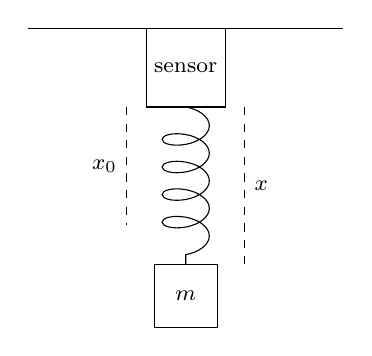
\begin{tikzpicture}
            \draw (-2,0) -- (2,0);
            \draw (-0.5,0) rectangle ++(1, -1) node [midway] {\footnotesize sensor};
            \draw[decorate, decoration={coil, segment length=3.5mm, amplitude=3mm}] (0,-1) -- ++(0, -2);
            \draw (-0.4,-3) rectangle ++(0.8, -0.8) node [midway] {\footnotesize $m$};
            \draw[dashed] (0.75,-1) -- ++(0, -2) node [midway, right] {\footnotesize $x$};
            \draw[dashed] (-0.75,-1) -- ++(0, -1.5) node [midway, left] {\footnotesize $x_0$};
        \end{tikzpicture}
    \end{minipage}
\end{frame}

\begin{frame}
    \frametitle{Materials and Methods}
    Length $L$ and displacement $x$ were measured using a meter stick. The mass
    $m$ was given on the mass itself. The force $F$ was measured using a force
    sensor. The angle $\theta$ was ensured to be less than \ang{15} using a
    protractor. The period $T$ was measured using a stopwatch. For the
    pendulum, four masses were tested for five trials each. For each trial,
    five periods were measured and averaged to reduce error. For the spring,
    four masses were tested for one trial each. For each trial, the initial and
    final displacement were measured.
\end{frame}

\begin{frame}
    \frametitle{Calculations}
    \begin{minipage}{0.35\textwidth}
        Pendulum:
        \begin{gather}
            a = -\omega^2x \\
            -\omega = \sqrt{\frac{a}{x}} \\
            \omega = \sqrt{\frac{g}{L}} = \frac{2\pi}{T} \\
            T = 2\pi\sqrt{\frac{L}{g}} \\
            T^2 = \frac{4\pi^2}{g}L \\
            \frac{4\pi^2}{T^2} = g\frac{1}{L}
        \end{gather}
        Spring:
        \begin{gather}
            F = kx \\
            kx = mg 
        \end{gather}
    \end{minipage}%
    \hspace{0.04\textwidth}%
    \begin{minipage}{0.6\textwidth}
        \centering
        \captionof{table}{Pendulum Example Calculations}
        \begin{tabular}{c|c|c|c}
            \toprule
            $L$ & $T$ & $\frac{1}{L}$ & $\frac{4\pi^2}{T^2}$ \\
            \midrule
            $0.58\si{\meter}$ & $1.46\si{\second}$ & $1.72\si{\per\meter}$ & $18.5\si{\newton}$ \\
            $0.36\si{\meter}$ & $1.18\si{\second}$ & $2.78\si{\per\meter}$ & $28.4\si{\newton}$ \\
        \end{tabular}
        \vspace{1cm}
        \captionof{table}{Spring Example Calculations}
        \begin{tabular}{c|c|c}
            \toprule
            $m$ & $x$ & $k \cdot x$ \\
            \midrule
            $0.1\si{\kilogram}$ & $0.043\si{\meter}$ & $1.00\si{\newton}$ \\
            $0.2\si{\kilogram}$ & $0.085\si{\meter}$ & $1.98\si{\newton}$ \\
        \end{tabular}
    \end{minipage}
\end{frame}

\begin{frame}
    \frametitle{Pendulum Graphical Relationship}
    \centering
    \begin{tikzpicture}
        \begin{axis}[
                xlabel={$\frac{1}{l}$ (\si{\per\meter})},
                ylabel={$\frac{4\pi^2}{T^2}$ (\si{\newton})},
                tick label style={/pgf/number format/fixed},
                scaled ticks=false,
                width=0.8\textwidth,
                legend pos=south east,
            ]
            \addplot +[only marks,mark size=1.5pt] table
            {pendulum.dat};
            \addplot table [
                y={create col/linear regression={y=y}},
                mark=none,
            ]
            {pendulum.dat};
            \addlegendentry{$\frac{4\pi^2}{T^2} = g\frac{1}{L}$}
            \addlegendentry{$\hat{\frac{4\pi^2}{T^2}} = \pgfmathprintnumber{\pgfplotstableregressiona}(\frac{1}{L})$}
        \end{axis}
    \end{tikzpicture}
\end{frame}

\begin{frame}
    \frametitle{Spring Graphical Relationship}
    \centering
    \begin{tikzpicture}
        \begin{axis}[
                xlabel={$m$ (\si{\kilogram})},
                ylabel={$kx$ (\si{\newton})},
                tick label style={/pgf/number format/fixed},
                scaled ticks=false,
                width=0.8\textwidth,
                legend pos=south east,
            ]
            \addplot +[only marks,mark size=1.5pt] table
            {spring.dat};
            \addplot table [
                y={create col/linear regression={y=kx}},
                mark=none,
            ]
            {spring.dat};
            \addlegendentry{$kx = m \cdot g$}
            \addlegendentry{$\hat{kx} = {m} \cdot \pgfmathprintnumber{\pgfplotstableregressiona}$}
        \end{axis}
    \end{tikzpicture}
\end{frame}

\begin{frame}
    \frametitle{Discussion}
    In the pendulum experiment, the data was very linear, with a $R^2$ value of
    0.97 and found a slope of $g = 10.5\si{\meter\per\second\squared}$. This
    value deviates from the accepted value of
    $9.8\si{\meter\per\second\squared}$ by 7\%. Error in this experiment could
    be due to the fact that the pendulum was not a perfect simple harmonic
    oscillator. The spring experiment had a $R^2$ value of 0.99 and found a
    slope of $k = 9.7\si{\newton\per\meter}$. This value deviates from the
    accepted value of $9.8\si{\newton\per\meter}$ by 1\%. Error in this
    experiment could be due to the fact that the measured k value was smaller
    than the actual k value of the spring.
\end{frame}

\end{document}
